% !TeX spellcheck = es_ES
\documentclass[12pt, titlepage]{article}
\usepackage[utf8]{inputenc}
\usepackage[spanish]{babel}
\usepackage{float}
\usepackage[letterpaper, margin=2.5cm]{geometry}
\usepackage[nottoc,notlot,notlof]{tocbibind} % Hace que se agregen las referencias al indice
\usepackage{url}
\usepackage{graphicx} 
\usepackage{listings}
\usepackage{color}
\definecolor{dkgreen}{rgb}{0,0.6,0}
\definecolor{gray}{rgb}{0.5,0.5,0.5}
\definecolor{mauve}{RGB}{253,151,31}

\lstset{frame=tb,
    language=Sql,
    aboveskip=3mm,
    belowskip=3mm,
    showstringspaces=false,
    columns=flexible,
    basicstyle={\small\ttfamily},
    numbers=none,
    numberstyle=\tiny\color{gray},
    keywordstyle=\color{blue},
    commentstyle=\color{dkgreen},
    stringstyle=\color{mauve},
    breaklines=true,
    breakatwhitespace=true,
    tabsize=2,
    morekeywords={use}
}

\title{Práctica 1}
\author{Carlos Tonatihu Barrera Pérez \\ Profesor: Hernández Contreras Euler \\ Bases de Datos \\ Grupo: 2CM1 }
\date{27 de febrero de 2017}

\begin{document}
    \maketitle
    \tableofcontents
    \section{Marco Teórico}
    Cosas mágicas
    \section{Desarrollo}
    En esta practica se comenzó creando la base de datos y seleccionándola para poder usarla.
    \begin{lstlisting}
    create database trabajos_terminales;
    use trabajos_terminales;
    \end{lstlisting}
    \begin{figure}[H]
        \begin{center}
            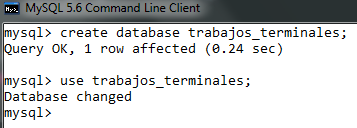
\includegraphics[width=14cm, height=6cm]{img/create.png}
            \caption{Creación y uso de la base.}
            \label{fig:create}
        \end{center}
    \end{figure}
    Se crearon las relaciones con las que se planeaba trabajar, el orden en el que se crean es importante para evitar errores.
    \begin{lstlisting}
    create table tt(
        nott int not null primary key,
        titulo varchar(100)
    );
    
    create table depto(
    idDepto int not null primary key,
    nombre varchar(50)
    );
    
    create table profesor(
        idProf int not null primary key,
        nombre varchar(20),
        ap varchar(30),
        am varchar(30),
        academia varchar(50),
        salario double,
        idDepto int,
        foreign key(idDepto) references depto(idDepto) on delete cascade on update cascade
    );
    
    create table presentacion(
        idPresentacion int not null primary key,
        fecha date,
        califRevisor float,
        califSinodales float,
        tipo varchar(30)
    );
    
    create table dirige(
        idProf int not null,
        nott int not null,
        primary key(idProf, nott),
        foreign key(idProf) references profesor(idProf) on delete cascade on update cascade,
        foreign key(nott) references tt(nott) on delete cascade on update cascade
    );
    \end{lstlisting}
    \begin{figure}[H]
        \begin{center}
            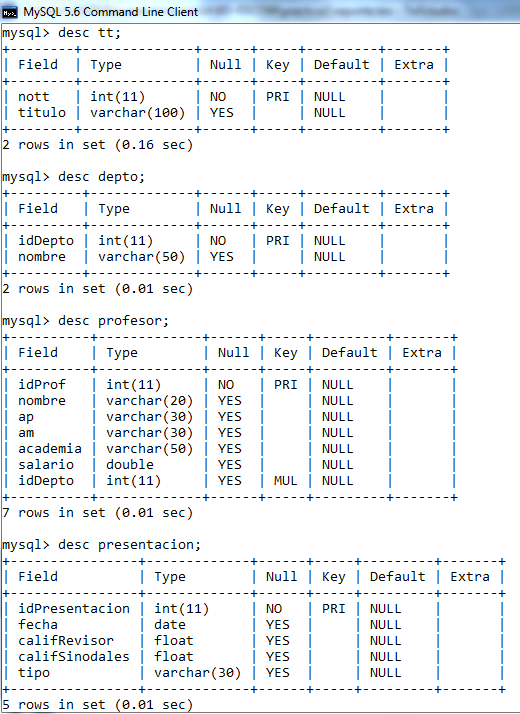
\includegraphics[width=16cm, height=14cm]{img/tablas.png}
            \caption{Descripción de las tablas.}
            \label{fig:tablas}
        \end{center}
    \end{figure}
    En este punto se empezó a modificar la descripción de las tablas
    \begin{lstlisting}
    alter table profesor rename as catedratico;
    alter table presentacion add column dictamen varchar(30);
    alter table depto change column nombre depto varchar(50) not null;
    alter table catedratico add column tel int;
    alter table catedratico change column tel tel varchar(30);
    \end{lstlisting}
    \begin{figure}[H]
        \begin{center}
            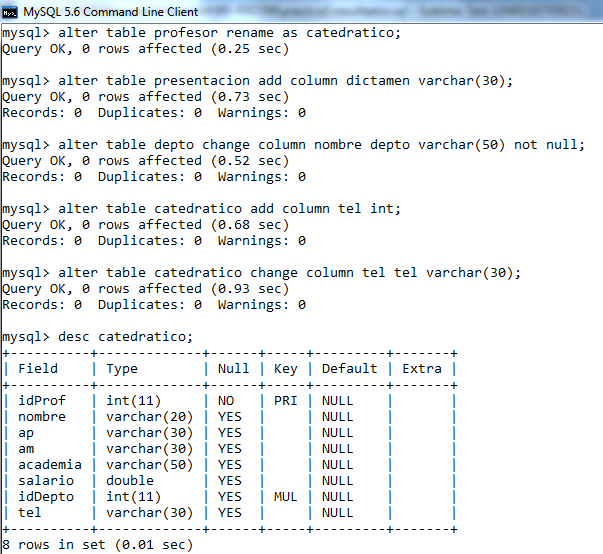
\includegraphics[width=14cm, height=9cm]{img/cambios.png}
            \caption{Cambios en la base.}
            \label{fig:cambios}
        \end{center}
    \end{figure}
\begin{figure}[H]
    \begin{center}
        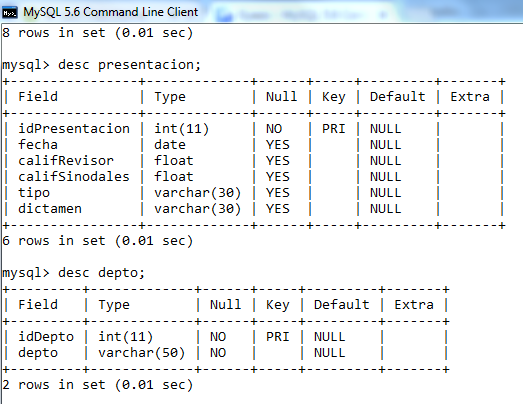
\includegraphics[width=12cm, height=6cm]{img/mascambios.png}
        \caption{Más cambios.}
        \label{fig:cambios2}
    \end{center}
\end{figure}
    Ahora se procedió a agregar una llave foránea a la tabla presentación, para esto primero se creo la columna que seria la futura FK y se especifica con que tabla tiene relación.
    \begin{lstlisting}
    alter table presentacion add column nott int;
    alter table presentacion add FOREIGN KEY(nott) references tt(nott)
    on delete cascade on update cascade;
    \end{lstlisting}
    \begin{figure}[H]
        \begin{center}
            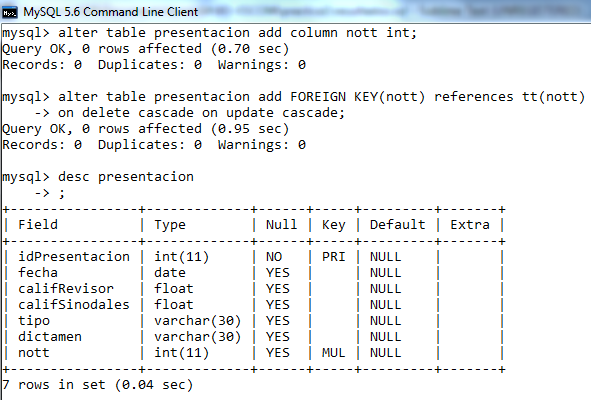
\includegraphics[width=12cm, height=6cm]{img/foranea.png}
            \caption{Creación de la llave foranea.}
            \label{fig:foranea}
        \end{center}
    \end{figure}
    Después se modifico la llave primaria haciéndola compuesta para lograr esto se borra la anterior PK y se agrega la nueva.
    \begin{lstlisting}
    alter table presentacion drop primary key;
    alter table presentacion add primary key(idPresentacion, fecha);
    \end{lstlisting}
    \begin{figure}[H]
        \begin{center}
            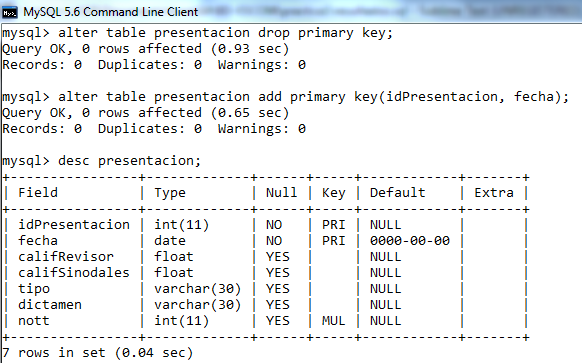
\includegraphics[width=12cm, height=6cm]{img/primaria.png}
            \caption{Creación de la llave primaria compuesta.}
            \label{fig:primaria}
        \end{center}
    \end{figure}
    Finalmente se elimino la clave foránea de una tabla, esto es mas complejo que la llave primaria ya que se debe observar la descripción de la relación para obtener el constraint que tiene asignado dicha clave.
    \begin{lstlisting}
    show create table catedratico;
    alter table catedratico drop foreign key catedratico_ibfk_1;
    \end{lstlisting}
    \begin{figure}[H]
        \begin{center}
            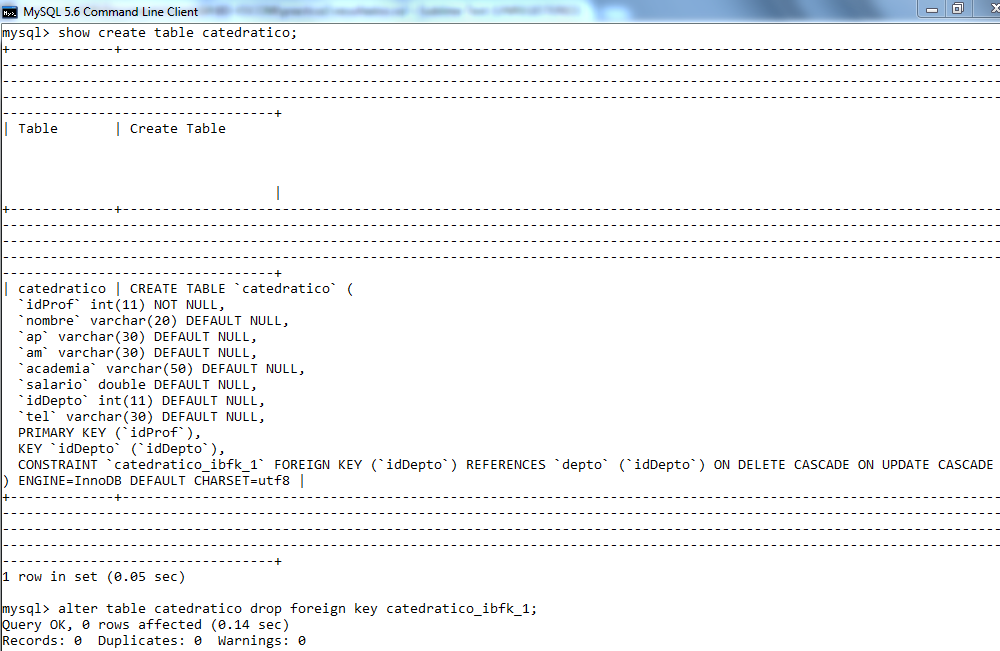
\includegraphics[width=16cm, height=10cm]{img/constraint.png}
            \caption{Se identifico y borro la clave foránea}
            \label{fig:constraint}
        \end{center}
    \end{figure}
\begin{figure}[H]
    \begin{center}
        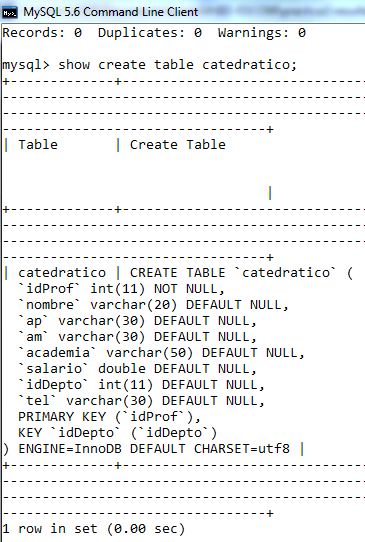
\includegraphics[width=10cm, height=12cm]{img/constraint2.png}
        \caption{Este fue el resultado de borrarlo.}
        \label{fig:constraint2}
    \end{center}
\end{figure}
    Para finalizar se hizo un respaldo, es importante estar en la ruta que se muestra en la imagen para poder realizar esto
    \begin{figure}[H]
        \begin{center}
            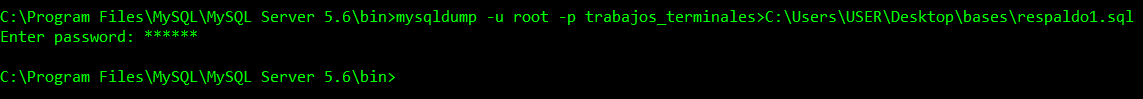
\includegraphics[width=16cm, height=3cm]{img/respaldo.png}
            \caption{Se logro hacer el respaldo sin errores.}
            \label{fig:respaldo}
        \end{center}
    \end{figure}
    \section{Conclusiones}
    Esta primera práctica me permitió empezar a conocer el como se trabaja con una base de datos a un nivel básico pero fundamental también es importante destacar que para dominar esta técnica es necesario seguir practicando y repasando las practicas que se hagan de aquí en adelante.
    \bibliography{bibliografia} 
    \bibliographystyle{ieeetr}
\end{document}